\documentclass[a4paper,12pt]{report}

\usepackage[frenchb]{babel}
\usepackage[utf8]{inputenc}
\usepackage[top=3cm, bottom=3cm, left=2.8cm, right=2.8cm]{geometry}
\usepackage{algorithm,algorithmic}
\usepackage{graphicx}


\title{Navigation dans un environnement 3D \vspace{0.5cm}}
\author{Marc BEYSECKER, Tom GIMENEZ, Valentin HIRSON, Léo RIZZON\\  \\Professeur encadrant : Mr Frédéric Koriche \\ \\Université Montpellier II \\  \\Master 1 Informatique}


\date{}
\begin{document}

\maketitle

\tableofcontents

\newpage

\chapter*{Remerciements}

Ma mère, ta mère. Merci mon cul bonsoir m'ssieurs dames.

\chapter{Introduction}


\section*{Contexte}

Dans les jeux vidéos, les personnages non joués par des humains doivent pouvoir se déplacer de manière autonome et cohérente. Un environnement 3D est constitué d'un graphe énorme avec des milliers de sommets. Même en ne prenant que le sol, le graphe est encore très gros et, surtout, n'est pas seulement constitué des points naviguables. C'est à dire que le personnage ne doit pas pouvoir se déplacer dessus.

Comme nous l'avons étudié, la recherche de chemins dans un graphe est un problème classique mais qui peut s'avérer très lourd sur de gros graphes. En prenant en compte que les jeux mettent en scène un grand nombre d'agents il s'agit de minimiser les temps de calculs. 

Il s'agit donc d'une part de ne sélectionner que les points naviguables et de simplifier le graphe obtenu pour limiter les espaces de calculs. De ces opérations nait le graphe de way-points. Il s'agit donc du graphe sur lequel vont se déplacer les agents.

Dans la plupart des jeux actuels les environnements sont créés ``à la main'' par les créateurs du jeu et les game designers placent eux même les points du graphe des way-points. Cela représente un gros travail et c'est même impossible dans le cas d'environnements aléatoirement générés.

Dans le cadre de notre unité d'enseignement intitulée Algorithmes de l'Intelligence Artificielle, nous avons réalisé un projet qui consiste en l'implémentation d'un algorithme de génération automatique du graphe des way-points.


\section*{Objectifs}

La base de notre travail est une scène 3D créée à l'aide d'un logiciel d'éditions d'objets 3D, par exemple Blender. Il s'agit alors de charger cette scène pour y appliquer nos traitements. Tout d'abord, il faut générer le graphe à partir de tous les points composant les différentes formes pour représenter les arêtes. Ensuite il faut épurer ce graphe pour ne garder que les sommets et les arêtes ``emruntables``. Enfin on va chercher à appliquer un algorithme de simplification pour ne garder que les points réellement utiles. C'est une procédure appelée merging.

Le résultat serait donc un graphe des way-points, simplifié, automatiquement généré.

\chapter{Recherches préliminaires}

\section{Une scène en 3D avec Blender}

Blender est un logiciel d'édition d'objets 3D libre sous licence GPL. Bien que nous ayons eu la possibilité d'utiliser des logiciels payant très évolués, nous avons fait le choix, approuvé par notre professeur encadrant, d'utiliser Blender. Blender est multi-platerformes et c'est cet aspect qui nous a décidé car nous travaillons tous sous Linux. Bien que gratuit, il offre largement toutes les fonctionnalités dont avions besoin.

\subsection{Le maillage}

Pour simuler le travail sur un terrain assimilable à un environnement 3D de jeux vidéo, il nous fallait un graphe avec beaucoup de points. L'objectif était de passer 

INSERER IMAGES CARRE SIMPLE PUIS MAILLAGE

Créer une scène simple sous Blender a été plutôt facile. Pourtant nous avons eu plus de mal à obtenir un maillage. Nous avons alors exploré plusieurs possibilités.

\paragraph{Une map Half-Life}

Au départ, nous avions dans l'idée de partir d'une map Half-Life. Dans un premier temps nous générions la map avec un générateur de terrain : Gensurf. Ensuite nous l'importions et l'éditions avec l'éditeur de map officiel WorldCraft. Nous arrivions donc à générer une scène rapidement et plus facilement qu'avec Blender. 
Malheureusement l'éditeur de map WorldCraft ne permet pas d'exporter directement en .obj , après quelques recherches, nous avons contourner le problème en utilisant Object Viewer qui permet de transformer un .map en .obj.

Au final, nous n'avons pas retenue cette solution car le .obj obtenu n'était pas aussi "propre" que celui obtenu par Blender. De plus la scène avait une épaisseur, ce qui ne nous plaisait pas.

\paragraph{La solution avec Blender}

Pour fabriquer notre sol nous avons longtemps cherché un modèle pré-conçu mais cela s'avéra infructueux.
Nous avons alors découvert qu'il était possible de diviser une forme de base. Nous avons décider de prendre un simple carré, de l'agrandir à la taille souhaitée et de le diviser en autant de petites cases que nécessaires. Cela nous a donc donné notre maillage sur lequel poser nos formes.
Nous avons posé des pavés sur notre sol car se sont les formes que prennent les bounding box. Une bounding box est la forme simplifiée que prend un modèle 3D; cela permet de simplifier les calculs d'intersection entre la forme et son environnement.

\subsection{Les différents formats de fichier}

Une fois la scène créée sous Blender le logiciel nous proposait différents format d'exportation. Il y en a un grand nombre et nous en avons étudié principalement deux.

\paragraph{COLLADA}

Collaborative Design Activity (abrégé en COLLADA, signifiant activité de conception collaborative) a pour but d'établir un format de fichier d'échange pour les applications 3D interactives.

COLLADA définit un standard de schéma XML ouvert pour échanger les acquisitions numériques entre différents types d'applications logicielles graphiques qui pourraient autrement conserver leur acquisition dans des formats incompatibles. Les documents COLLADA, qui décrivent des acquisitions numériques, sont des fichiers XML, habituellement identifiés par leur extension .dae («digital asset exchange», traduit par «échange numérique d'acquisition»).
C'est un format supportant la vaste majorité des fonctionnalités modernes
requises par les développeurs de jeux vidéo. 

Il fallait donc faire un choix, COLLADA étant plus conséquent que .obj, et le sujet de notre TER n'étant pas porté sur le format de notre scène, 
nous avons donc choisi de faire simple et de choisir .obj. De plus le format XML nous obligeait à utiliser des librairies dédiées, complexes et non standardisées, qui nous aurait pris beaucoup plus de temps pour écrire le parser.

\paragraph{WaveFront}

OBJ est un format de fichier contenant la description d'une géométrie 3D. Il a été défini par la société Wavefront Technologies. Ce format de fichier est ouvert et a été adopté par d'autres logiciels 3D (tels que Maya, 3D Studio Max, Lightwave et bien sur Blender) pour des traitements d'import / export de données.

Dans un fichier Wavefront (extension .obj), les formes sont stockées les unes après les autres. Les différentes entités sont écrites par bloc.
Donc, pour chaque forme les informations qui la concerne sont stockées ligne par ligne. Nous savons à quoi chaque information correspond grace à la lettre clef qui débute la ligne ( par exemple: ''v'' pour un vertex ).
Les seuls informations qui nous intéressent sont les vertex et les faces. 
Une ligne pour un vertex fournit la position de ce vertex (x, y, z) écrit comme suit ''v x y z'' par exemple ''v 2.0 2.0 3.0'' pour un vertex de coordonnées (2.0, 2.0, 3.0)
Une ligne pour une face fournit le numéro des vertex qui la composent écrit comme suit ``f num$_{1}$ ... num$_{n}$`` par exemple ``f 4 6 7 8 11 13``pour une face constituée des vetices numéros 4, 6, 7, 8 et 11. Le numéro d'un vertex n'est pas explicitement donné mais il se déduit par son ordre d'apparition dans le fichier Wavefront. C'est un identifiant unique.

Voici un exemple de code dans un fichier .obj.

Ici il s'agit d'un simple carré. Une forme commence par la liste des points qui la constitue puis la liste de ses faces.

\begin{verbatim}
v 0 0 0 //premier point de la nouvelle forme
v 0 0 1
v 1 0 1
v 1 0 0
f 1 2 3 4 //première face constituée des points 1 2 3 4
v ... //un v après un f on est donc sur une nouvelle forme
\end{verbatim}

Nous avons donc choisi ce format de fichier pour stocker notre scène 3D car il nous a été très facile de développer le parser adéquat. Les informations fournies sont justes celles dont nous avons besoin. On peut noter toutefois qu'il est possible d'exporter également des données sur les textures et les normales mais nous n'utilisons pas ces fonctionnalités.

\section{Récupérer notre scène en 3D}
 
Une fois notre scène créée sous Blender s'est posé le problème de l'exploiter. Nous avons alors cherché du côté des librairies existantes, en C/C++ surtout. En effet, Blender nous proposait divers format de fichier de sortie. Nous devions faire en sorte que les informations soient récupérables et exploitable pour nos algorithmes. L'idée générale est d'utiliser un parser qui va lire les données du fichier pour les transformer en données compréhensibles par notre programme.

Voici les solutions que nous avons envisagées.
 
\subsection{OpenSceneGraph}

\subsection{OpenGL avec nos propres structures de données}

Une fois l'expérience OpenSceneGraph terminée et mise de côté, nous avons dû de nouveau chercher une solution. Après de longues recherches, nous avons trouvé quelques possibilités comme OGRE (Object-Oriented Graphics Rendering Engine), nous avons finalement décidé de créer nous même ce dont nous avions besoin. C'est la solution finale.

L'utilisation d'OpenGL, conseillée par notre professeur encadrant, était un choix établi. Libre et accessible, OpenGl est de plus au programme de l'année prochaine : il est toujours intéressant de prendre un peu d'avance. OpenGL nous sert à afficher notre scène 3D.

Coder en C++, pour la performance du programme, pour l'aspect objet intéressant dans notre contexte, pour l'utilisation d'OpenGL, était presque évident.

Finalement nous avons donc implémenté notre propre parser pour remplir nos propres structures de données. En fait, on a recodé une partie des fonctionnalités des librairies que nous avions étudiées pour n'en garder que ce dont nous avons besoin et pour avoir des structures que nous maitrisons pleinement. Au final, cela nous a fait gagné du temps.


\chapter{Implémentation finale}

Nous présenterons ici les éléments que nous avons effectivement implémentés.

\section{Principe général}

Voici le principe général de notre programme. Ci-après les différentes étapes successives en considérant que l'on part d'une scène 3D en format WaveFront.

\begin{itemize}
 \item Parser le fichier .obj de la scène 3D
 \item Isoler le sol des autres formes
 \item Générer le graphe correspondant au sol
 \item Détecter les sommets invalides et les retirer du graphe
 \item Simplifier le graphe (merging)
\end{itemize}

\section{Nos structures de données}

Nous présenterons ici nos structures de données, utilisées dans notre projet. Comme dit précédemment, nous avons exploité le potentiel objet du C++.

\begin{itemize}
 \item Forme:

Une \textit{forme} est une figure géométrique qui contient une liste de vertex et une liste de faces. À partir d'une forme, nous pouvons générer un graphe qui lui correspond.
 
 \item Vertex:

Un \textit{vertex} est un point de notre scène. Il possède 3 coordonnées x, y et z. Il contient également une liste de pointeurs sur les vertices qui sont ses voisins.

 \item Faces:

Les \textit{faces} possèdent une liste contenant les numéros des vertex qui les composent. C'est grâce aux faces que nous pouvons déduire les voisins des sommets du graphe. Elles servent aussi à effectuer un affichage cohérent des formes.

 \item Bounding Box:

\end{itemize}


\subsection{La scène}

Reprécisons bien comment sont stockées les données.

Notre scène, c'est à dire l'ensemble de tous les vertices et de toutes les formes, est stockée dans une liste de formes. On a donc, comme expliqué plus haut, une scène complète séparée en différentes formes : par exemple une forme qui correspond à tout le sol, une à un cube etc.

C'est pourquoi nous avons une méthode qui permet d'identifier quelle forme est le sol. Dans notre cas, nous avons pu faire très simple et la forme correspondant au sol est celle qui possède le plus de points.

\subsection{Le graphe géneré}

Pour stocker notre graphe dont la création est expliquée plus loin, nous avons fait le choix de rajouter à notre classe Vertex une liste d'adjacence contenant des pointeurs vers les voisins de ce sommet. C'est donc une méthode d'implémentation classique où chaque sommet connait ses voisins. Encore une fois, comme le point principal du projet n'est pas là, nous avons choisi de faire au plus simple. 

Grâce à cette liste de voisins (ou d'adjacences), les parcours dans le graphe sont possibles (cette liste représente les arêtes du graphe). Nous avons choisi les listes de voisins car chaque sommet possède au plus 4 voisins si le maillage est fait de carrés ou 3 voisins s'il est fait de triangles. Ce qui permet un coût de stockage très faible et un temps de calcul bien maitrisé. 

Prenons l'exemple de la suppression d'un voisin :

Il suffit de l'isoler pour qu'il ne soit plus parcouru ; soit le supprimer de la liste de voisins de tous ses voisins. Au pire des cas: 4 x 4 tests.
 
Cette liste d'adjacence est donc remplie à l'appel de la méthode de génération du graphe.

\section{Un parser pour récupérer notre scène}

Nous récupérons donc un fichier au format WaveFront. Il s'agit de remplir nos structures de données, un vecteur de forme que nous appelerons ici \textit{listeDeFormes}.
Nous avons présenté précédemment la structure d'un fichier au format WaveFront. Ici nous présenterons le fonctionnement de notre parser.

\begin{algorithm}[h]
\caption{Parser de fichier .obj}
\label{parser}
\begin{algorithmic}[1]
\REQUIRE fichier .obj
\FOR{chaque forme (c'est à dire une apparition de ''v`` après une série de ''f'')}
  \IF{la ligne commence par un ``v''}
    \STATE enregister ``v x y z'' comme nouveau vertex de coordonnées (x,y,z) dans le vecteur de vertex de la forme courante
  \ELSE
    \IF{la ligne commence par un ``f''}
    \STATE enregistrer ``f $x_{1}$ ... $x_{n}$'' comme nouvelle face dans le vecteur de faces de la forme courante
    \ENDIF
  \ENDIF
\ENDFOR
\end{algorithmic}
\end{algorithm}

\section{Génération du graphe correspondant au sol}

Pour effectuer les traitements prévus nous avons donc décider de travailler sur un graphe. Nous partons d'un ensemble de points et de faces dans des formes séparées. Nous selectionnons la forme correspondant au sol avec notre méthode dédiée. Ensuite, sur cette forme nous appliquons une méthode qui va créer les liaisons entre sommets en fonction des faces de la forme. 

Pour chaque face on lie ses vertices de manière à ce que chaque sommet prenne comme voisins son prédecesseur et son successeur dans leur ordre d'apparition de la liste des points de la face.

Notre sol n'est composé que de carrés et chaque face possède une liste de 4 sommets A,B,C,D.
voisins(A) = {B,D} ;  voisins(B) = {A,C} ; voisins(C) = {B,D} ; voisins(D) = {A,C}

\section{Travaux effectués sur le graphe}

Notre scène est donc récupérée dans notre programme. Nous avons de plus généré le graphe du sol. Il nous faut maintenant y appliquer nos traitements.

\subsection{Création du graphe des way-points}

Dans un premier temps, à partir de tous les points du graphe, nous allons chercher à supprimer tous les point sur lesquels un agent ne doit pas pouvoir se déplacer. Nous obtiendrons ainsi le graphe des way-points, ensemble des points navigables.

\subsubsection{Parcours}

Voici notre méthode de parcours, en profondeur. 

\begin{algorithm}[h]
\caption{Parcours du graphe complet : parcourir(sommet)}
\label{parcours_graphe}
\mbox{Algorithme lancé à partir d'un sommet non isolé}
\begin{algorithmic}[1]
\IF{sommet courant non marqué}
  \STATE marquer le sommet courant
  \FOR{chaque voisin v}
    \STATE parcourir(v)
  \ENDFOR
\ENDIF
\end{algorithmic}
\end{algorithm}

\subsubsection{Heuristique}

Notre heuristique, qui va déterminer si un point est naviguable ou pas va se baser sur les bounding box. Une bounding box est la plus petite boite englobant l'ensemble des points d'une forme. Générer une bounding box pouvant être un travail compliqué, nous avons choisi de dire que notre bounding box était constitué de quatres points (vertex). On calcule leurs coordonnées selon les valeurs minimales et maximales de tous les vertex d'une forme. On classe les quatres points afin de facilité les calculs à venir.

On considère comme valide :
\begin{itemize}
 \item un sommet s'il n'est pas contenu dans une bounding box. 
 \item une arête, entre deux sommets, si elle ne coupe pas une bounding box
\end{itemize}

Une arête, entre deux sommets, est valide si elle ne coupe pas une bounding box. Il nous a donc fallu implémenter deux méthodes renvoyant un prédicat pour savoir quels points et quelles arêtes supprimer. 
Quand un point est non valide, on l'isole dans le graphe. On peut afficher tous les points, voir clairement les diffétences. Le parcours du graphe est quand a lui simplifié.

L'heuristique a été un pilier très important de ce projet et a été l'objet d'une réflexion assez poussée. Nous présenterons différentes méthode qui ont été envisagées.

\paragraph{Méthode 1 }
Cette solution, souvent utilisé en informatique, consiste à déterminer si un point (x,y) est à l'intérieur ou à l'extérieur d'un
polygone sur un plan 2D. 
Considérons un polygone, fait de n sommets (x$_{i}$,y$_{i}$) avec $i$ de $0$ à $n-1$. Le dernier sommet (x$_{n}$,y$_{n}$) est le même que le premier sommet, pour que le polygone soit fermé. 
Pour déterminer le status d'un point (x$_{p}$,y$_{p}$), on trace une droite horizontale partant de (x$_{p}$,y$_{p}$). 
Si le nombre d'intersection de la droite avec chaque arête du poylygone est impaire alors le point est à l'intérieur du polygone, sinon il n'est pas dedans.

\begin{figure}[h]
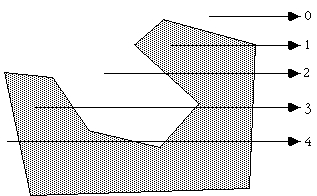
\includegraphics[scale=0.6]{Images/insidepoly1.jpg}
\includegraphics[scale=0.6]{Images/insidepoly3.jpg}
\caption{Différents cas de figures avec nombre d'intersection paire et impaire}
\label{nbintersect}
\end{figure}
\vspace{0.5cm}

Le seul problème apparait lorsqu'un sommet ou une arête du polygone est parallèle à la droite.

Les situations possibles sont illustrées en dessous :

\begin{figure}[h]
\centering
\includegraphics[scale=0.6]{Images/insidepoly2.jpg}
\caption{Illustration des épaisseurs de ligne}
\end{figure}
\vspace{0.5cm}

Les lignes épaisses ne sont pas considérées comme valides, les lignes fines si.
Il est bon de noter que cet algorithme marche avec des polygones troués, comme illustré sur le figure \ref{nbintersect}.

DESSIN

Cette méthode est idéale pour les polygones non convexes mais comme nous utilisons des carrés, elle aurait été un peu lourde.

\paragraph{Méthode 2 }
Une autre solution, est de calculer la somme des angles fait entre le point test et chaque paires de points du polygone. Si la somme est égale à $2\pi$ alors le point est à l'intérieur, sinon le point est à l'extérieur. 
Cette méthode marche aussi avec les polygones troués.
De même cette méthode est assez gourmande en calcul et n'a pas été retenue.

\paragraph{Méthode 3 : retenue}
La dernière solution que nous avons testé ne marche qu'avec les polygones convexes. Si un polygone est convexe alors on peut considérer ces arêtes comme un "chemin" partant du premier sommet pour y revenir. 
Un point est à l'intérieur du polygone si il est toujours du même côté que tous les arêtes constituant le "chemin".

\begin{figure}[h]
\centering
\includegraphics[scale=0.6]{Images/chemin2.jpg}
\caption{Un chemin dans un carré}
\end{figure}
\vspace{0.5cm}

Soit un segment entre P0(x$_{0}$,y$_{0}$), P1(x$_{1}$,y$_{1}$) et un autre point P(x,y) alors on a la relation suivante : (y - y$_{0}$).(x$_{1}$ - x$_{0}$) - (x - x$_{0}$).(y$_{1}$ - y$_{0}$).
Si le résultat est inférieur à 0 alors P est à droite du segment [P0,P1], si il est égale à 0 alors il est sur la droite (P0,P1) et s'il est supérieur à 0 alors il est à droite du segment [P0,P1].

A noter que cet algorithme ne marche pas avec les polygones troués. 

Il nous suffit donc de faire 4 tests, on teste la position du point par rapport à chacune des arêtes constituant le polygone, si le point est toujours du même côté alors le point est à l'intérieur du polygone.

Nous avons choisi de retenir la solution 3 car c'est celle qui nous semblait marcher le mieux ainsi que la plus économe en ressources. Elle est parfaitement adaptée à notre projet.

\paragraph{Méthode de test d'intersection d'une arête avec une bounding box }


Pour tester si une arête coupe une bounding box nous avons décomposé le problème :
\begin{itemize}
 \item dans un premier temps il nous fallait une méthode pour savoir si un segment est coupé par un autre.
 \item ensuite il suffit de tester si notre arête coupe chaque segment de la bounding box, notre bounding box étant un carré on a donc 4 tests à faire.
\end{itemize}

L'intersection d'un segment avec un autre peut être un problème extrêment simple ou extrêment compliqué, dépendant de l'application. 
Mais si l'on veut seulement le point d'intersection alors la méthode suivante marche :

Soit A,B,C,D des vecteurs. Alors on a les propriétés suivantes :

$AB=A+r(B-A)$, $r \in [0,1]$

$CD=C+s(D-C)$, $s \in [0,1]$

$r = \frac{(A_{y}-C_{y})(D_{x}-C_{x})-(A_{x}-C_{x})(D_{y}-C_{y})}{(B_{x}-A_{x})(D_{y}-C_{y})-(B_{y}-A_{y})(D_{x}-C_{x})} (eqn 1)$

$s = \frac{(A_{y}-C_{y})(B_{x}-A_{x})-(A_{x}-C_{x})(B_{y}-A_{y})}{(B_{x}-A_{x})(D_{y}-C_{y})-(B_{y}-A_{y})(D_{x}-C_{x})} (eqn 2)$

Après, le test est simple : 
\begin{itemize}
 \item Si $0\le r \le 1 \wedge 0 \le s \le 1 \rightarrow$ intersection
 \item Si $r<0 \vee r>1 \vee s<0 \vee s>1 \rightarrow$ pas d'intersection
\end{itemize}

\subsection{Simplification du graphe des way-points : merging}

Pour limiter les calculs de recherche de chemins les graphes des way-points sont généralement simplifier par l'application d'une technique qu'on appelle merging. 

Nous n'avons pas eu le temps de développer un merging très évolué. Toutefois notre procédure de merging remplit son oeuvre en préservant la connexité du graphe. Il s'agit en fait d'isoler certain sommets dont l'entourage possède un grand nombre de voisins. 

\begin{algorithm}[h]
\caption{Merging du graphe : merging(sommet)}
\label{merging_graphe}
\mbox{Algorithme lancé à partir d'un sommet non isolé}
\begin{algorithmic}[1]
\IF{sommet courant non marqué}
  \STATE dupliquer la liste des voisins
  \IF{sommet courant a 4 voisins}
    \IF{sommets voisins du sommet courant ont tous au moins 3 voisins}
      \STATE isolation du sommet courant
    \ENDIF
  \ENDIF
  \FOR{chaque voisin v sauvegardé}
    \STATE merging(v)
  \ENDFOR
\ENDIF
\end{algorithmic}
\end{algorithm}

\begin{figure}[h]
\centering
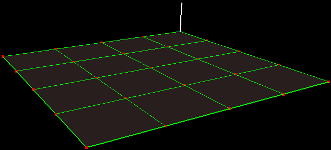
\includegraphics[scale=0.6]{Images/maillage.png}
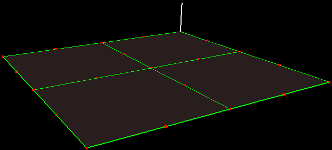
\includegraphics[scale=0.6]{Images/merging.png}
\caption{Notre graphe avant et après merging}
\end{figure}
\vspace{0.5cm}

\chapter{Résultats}

\section{Interface graphique}
commandes

\section{Application de l'heuristique}
screenshot

\section{Merging}
screenshot

\section{Déplacement d'un agent}



\chapter{Bibliographie}

\section*{OpenSceneGraph}
\section*{OpenGL}
\section*{Le langage C/C++}
\section*{Blender}
\section*{WaveFront (.obj)}
\section*{SDL}
\section*{Ogre}
\section*{Map to obj}
\section*{Bounding Box}

\chapter{Conclusion}

\subsection*{Bilan technique}

\subsection*{Bilan personnel}

\end{document}
